\chapter{引言}
\label{chap:introduction}

\section{粒子物理中的标准模型}
1964 年,美国物理学家盖尔曼(Murray Gell-Mann)和兹韦格(George Zweig)分别提出了夸克模型~\cite{c1_qmodel_gell,c1_qmodel_Zweig},
他们认为,质子、中子等强子并不基本,而是由更基本的粒子--夸克组成的。他们认为强子由以下三种夸克组成:上夸克($u$)、下夸克($d$)及奇异夸克($s$)。
这种三夸克模型很好地解释了当时已发现的强子和共振态粒子,并成功预言了一些未发现粒子。 
也得到了后来进行的高能电子、高能中微子对质子和中子的深度非弹性散射实验的支持,实验显示出质子和中子内部存在点状结构,这些点状结构可以认为是夸克存在的证据。

到目前为止实验上尚未发现轻子和夸克还有内部结构。人们相信轻子是与夸克属于同一层次的基本粒子。
理论和实验上最终表明不可再分的基本粒子可以归为三代,具体可以参看表\ref{tab:fermion}。
夸克(上夸克$u$与下夸克$d$、粲夸克$c$与奇夸克$s$、顶夸克$t$与底夸克$b$,以及它们的反粒子)和三代轻子(电子$e$、缪子$\mu$、陶子$\tau$ 以及对应的中微子$\nu_e$、$\nu_{\mu}$、$\nu_{\tau}$,并且还有它们的反粒子),以及传播强相互作用的传播子胶子、传播弱相互作用的传播子$W^{\pm}$和$Z^0$玻色子、传播电磁相互作用的光子、另外一个为解释质量起源的Higgs粒子,从而搭建了当代粒子物理学最成功的理论模型--标准模型(图\ref{fig:SM}和表\ref{tab:SM})。

现在一般意义上的标准模型理论指的就是电弱统一理论和量子色动力学(QCD)的统称。一般可以抽象为如下群表示SU(3)$_{C}$$\times$SU(2)$_{L}$$\times$U(1)$_{Y}$,其中SU(3)$_{C}$指代的是强相互作用,$C$指的是颜色,表示强相互作用只发生在带有色量子数的粒子之间;SU(2)$_{L}$$\times$U(1)$_{Y}$指代的是电弱相互作用,$L$指的是只有左手的粒子参与,$Y$代表超荷。标准模型是迄今为止公认的描述弱、电、强三种相互作用的成功理论。四十多年来,标准模型经历了各种实验的精确检验,取得了巨大的成功。

\begin{figure}[!tbp]
 \centering
 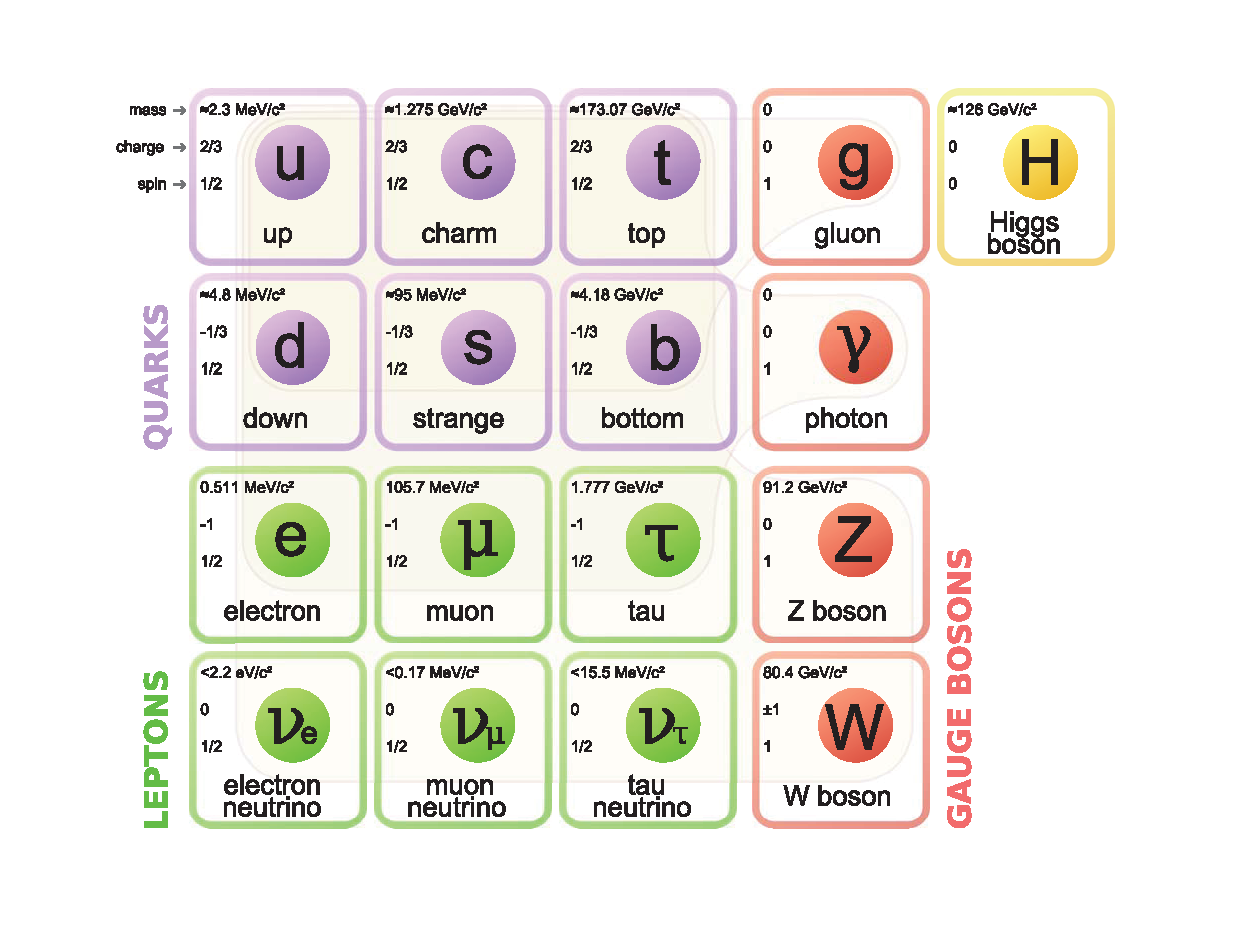
\includegraphics[width=0.8\textwidth]{chap1_SMparticles.pdf}
 \caption{粒子物理的标准模型。}
 \label{fig:SM}
\end{figure}

\begin{table}
\centering
\caption{标准模型中的三代费米子。}
%\begin{tabular*}{40cm}{llllll}
\begin{tabular}{lllll}
\toprule
&  \multicolumn{3}{c}{味道} & 电荷     \\
	\midrule
\multirow{2}*{轻子}  & $e$ & $\mu$ & $\tau$   &     -1       \\
& $\nu_{e}$ & $\nu_{\mu}$ & $\nu_{\tau}$   &     0       \\
\multirow{2}*{夸克}  & $u$ & $c$ & $t$   &     +$\frac{2}{3}$       \\
& $d$ & $s$ & $b$   &     -$\frac{1}{3}$       \\
\bottomrule
%\end{tabular*}
\end{tabular}
\label{tab:fermion}
\end{table}

\begin{table}
\centering
\footnotesize
\caption{四种玻色子及其性质。}
%\begin{tabular*}{40cm}{llllll}
\begin{tabular}{lllllll}
\toprule
名称 & 相互作用 & 自旋/宇称  & 力程(m) & 作用强度 & 典型作用时间(sec) & 理论描述  \\
	\midrule
胶子            & 强相互作用   & $1^{-}$       &  $10^{-15}$ &  1          &  $10^{-23}$  & 量子色动力学(QCD)   \\
光子            & 电磁相互作用 & $1^{-}$       &  $\infty$   &  $10^{-2}$  &  $10^{-16}$  & 量子电动力学(QED)   \\
$W^{\pm},Z^{0}$ & 弱相互作用   & $1^{-},1^{+}$ &  $10^{-18}$ &  $10^{-5}$  &  $10^{-10}$  & 量子味动力学(QFD)   \\
引力子          & 引力相互作用 & $2^{+}$       &  $\infty$   &  $10^{-39}$ &  $---$        & 广义相对论   \\
\bottomrule
%\end{tabular*}
\end{tabular}
\label{tab:SM}
\end{table}


\section{粲重子$\lambdacp$强子衰变分支比}

$\lambdacp$的质量约为质子质量的2.5倍,质量差别主要来自质子中的上夸克换成了较重的粲夸克。
粲重子$\lambdacp$作为最轻的粲重子,包含三个夸克, 即由一个重的粲夸克和两个处于同位旋$I$=0的轻夸克($u,d$)组成,如图\ref{fig:lambdac_quark}所示。
粲夸克弱衰变几乎主导了$\lambdacp$的衰变模式。
研究$\lambdacp$衰变不仅可以用来检验弱作用理论,更重要的是可以利用粲重子的跃迁来检验强相互作用机制,比如$\lambdacp$内部三个夸克的分布及相应动力学机制、以及强相互作用的SU(3)对称性等。
粲重子$\lambdacp$内部既有重夸克,又有轻夸克,因此,有其特别值得研究的地方。
这样的系统既具有重夸克对称性,又具有轻夸克手征对称性。
重夸克有效理论认为:当重夸克质量趋近无限大时,重夸克与轻夸克的自旋将退耦,重子的性质完全由轻夸克的自由度决定。
这就是通常所说的重-轻系统满足的重夸克对称性。
另外,对于较轻的$u$、$d$夸克,在取其质量为0的极限下,QCD的拉氏量具有SU(3)$_{L}$$\times$SU(3)$_{R}$的整体对称性,称为手征对称性。
研究粲重子可以很好的理解轻夸克在重夸克环境下的动力学行为, 很好的检验重夸克对称性和轻夸克手征对称性, 这对理解低能区重子和Goldstone玻色子之间的相互作用至关重要。
如图\ref{fig:charmed_baryon}所示,很多高激发态粲重子最终都要衰变到处于基态的$\lambdacp$。
不仅如此,含底夸克的$\Lambda_b$重子和$B$介子也会衰变到含$\lambdacp$末态,对$\lambdacp$衰变性质的研究也有助于进一步理解重味重子谱学及其衰变性质。
对于主要由底夸克衰变主导的实验,测量每一个底夸克产生的粲夸克数目(charm counting)以及测量唯象描述夸克强子化过程的碎裂函数,可以很好的对QCD进行检验~\cite{Abreu:1999vw,Barate:1999bg}。
而测量$\lambdacp$的强子衰变分支比对于此类问题是个重要输入量。
目前对于此类计算最大的系统误差来源已经是粲重子$\lambdacp$的衰变分支比~\cite{Dytman:2002yd,Aaij:2011jp}。

\begin{figure}[!tbp]
\begin{center}
\includegraphics[width=0.85\textwidth]{chap1_Lambda_c_quark.pdf}
\end{center}
\caption{粲重子$\lambdacp$的夸克组分示意图。}
\label{fig:lambdac_quark}
\end{figure}

\begin{figure}[!tbp]
\begin{center}
\includegraphics[width=0.85\textwidth]{chap1_charmed_baryon.pdf}
\end{center}
\caption{粲重子及其高激发态重子跃迁示意图。}
\label{fig:charmed_baryon}
\end{figure}


\subsection{$\lambdacp$ 强子衰变的相关理论现状}

描述重子结构及其性质较为成功的两个理论就是所谓的重夸克有效理论(HQET)和夸克-双夸克模型(quark-diquark)。
重夸克有效理论~\cite{Georgi:1991ch,Neubert:1993mb}是理论物理学中的一个重要工具,理由很简单:对于物理问题的理解,考虑完全的理论往往是不必要的,在一个恰当的层次上来考虑问题反而会更加行之有效。
HQET是重夸克与轻自由度直接通过软胶子交换而形成相互作用的一个简单描述。
其中重夸克的质量$m_{Q}$是一个重要的能量标度。
HQET在预言某些强子的性质时,对于重夸克质量$m_{Q}$远大于轻夸克$u,d,s$的质量情况,选择$m_{Q}\to \infty$作一个近似计算。
这时的重夸克表现的像一个色三态的静外场源,强子内动力学可以约化为轻自由度和色场源的相互作用。
然而,实际上重夸克质量并不是无限大的,尤其我们讨论的粲重子中的$c$夸克的质量并不是特别的大,因此HQET理论在这种情况下需要对除领头阶之外的其余各项做高阶修正。
重子结构的夸克-双夸克模型是Lichtenberg等~\cite{Lichtenberg:1967zz}提出的。
后来很多作者讨论过夸克-双夸克模型,虽然细节各不相同,但这些工作多少都采用了这样一个相同的物理图像。
在重子内部,有两种组分夸克和双夸克,双夸克是两个夸克的束缚态,并与第三个夸克相互作用形成重子。
对于含有两个重夸克和一个轻夸克的重子,这两个重的夸克可以组合成一个所谓的双夸克。
如果含有一个重夸克和两个轻夸克的,则这两个轻的夸克更容易形成双夸克。
双夸克模型很久以前就已经被很多理论的文章采用,计算了很多涉及重子的过程~\cite{Anselmino:1987vk, Kroll:1987pj,Mannel:1990vg,Leinweber:1993nr,Ebert:1995fp}。
它有着明显的优点,化三体问题为两体问题,使计算大为简化。
用这一模型讨论重子介子散射、重子磁矩以及定性地讨论重子质量方面取得了一些成功。


具体到理论方面的计算。
介子和重子所有的非轻子衰变都可以归为如下几类的拓扑图: W外发射,W内发射,W交换图,W湮灭图和W圈图。
图\ref{fig:feynman_lambdapip}给出了粲重子$\lambdacp\to \Lambda \pip$衰变过程的三种典型拓扑图(W外发射,W内发射和W交换),其它衰变过程的图像大多与此类似的。
粲重子$\lambdacp$的衰变中是没有湮灭图贡献的。
我们研究的Cabibbo 允许的过程也不会出现圈图的贡献。
对于W内发射和外发射图通常认为是可因子化部分~\footnote{ W内发射意味着W出来的两个夸克要和其余夸克进行强子化,因此会有所谓的色压低效应。},而对于W交换和W湮灭图是不可以因子化的。
粲重子中的W内发射对可因子化提出了更高的要求,即通过弱衰变来的夸克要强子化成介子的情形才可以因子化,而强子化成重子的过程是不可以因子化的。
图\ref{fig:feynman_pK0bar}给出了粲重子$\lambdacp\to p \overline{K}{}^{0}$衰变过程的两个可能拓扑图(W内发射和W交换)。
我们可以清楚的看到图\ref{fig:feynman_lambdapip_C}中$s$夸克出现在重子$\Lambda$中,故该拓扑图是不可因子化的,而图\ref{fig:feynman_pK0bar_C}中$s$夸克是出现在介子$\overline{K}{}^{0}$中,故可以简单地认为该图是可以因子化的(后面会看到也有不可因子化的贡献)。

\begin{figure}[!tbp]
 \centering
\subfigure[W外发射T图]
{
 \includegraphics[width=0.3\textwidth]{chap1_feynman_lambdapi_external.pdf}
 \label{fig:feynman_lambdapip_T}
}
\subfigure[W内发射C图]
{
 \includegraphics[width=0.3\textwidth]{chap1_feynman_lambdapi_internal.pdf}
 \label{fig:feynman_lambdapip_C}
}
\subfigure[W交换E图]
{
 \includegraphics[width=0.3\textwidth]{chap1_feynman_lambdapi_exchange.pdf}
}
 \caption{粲重子$\lambdacp \to \Lambda\pip$衰变的典型拓扑图。}
 \label{fig:feynman_lambdapip}
\end{figure}

\begin{figure}[!tbp]
 \centering
\subfigure[W内发射C图]
{
 \includegraphics[width=0.4\textwidth]{chap1_feynman_pK0bar_internal.pdf}
 \label{fig:feynman_pK0bar_C}
}
\subfigure[W交换E图]
{
 \includegraphics[width=0.4\textwidth]{chap1_feynman_pK0bar_exchange.pdf}
}
 \caption{粲重子$\lambdacp \to p \overline{K}{}^{0}$衰变的典型拓扑图。}
 \label{fig:feynman_pK0bar}
\end{figure}

%由于理论上对于粲重子的计算还非常有限,我们尝试对应粲介子中的计算情况对粲重子的对应情况先进行一个相应的讨论:
众所周知,粲介子中不可因子化的W交换过程存在着色压低和螺旋度压低,与可因子化的发射图贡献相比,可因子化部分是占主导地位的。
简单因子化方法将外发射(图\ref{fig:feynman_lambdapip_T})和内发射(图\ref{fig:feynman_pK0bar_C},区别于图\ref{fig:feynman_lambdapip_C})贡献$a_{1}$,$a_{2}$分别写为~\cite{Fusheng:2011tw,Li:2012cfa}:
\begin{equation}
a_1(\mu)=C_2(\mu)+\frac{C_1(\mu)}{N_c},
a_2(\mu)=C_1(\mu)+\frac{C_2(\mu)}{N_c},
\end{equation}
$C_{1,2}$称作威尔逊系数,可以通过微扰论进行计算,$N_{c}$在因子化方法中指的是颜色的数目3。
其中$\mu=\sqrt{\Lambda m_D (1-r_1^2)(1-r_2^2)}$为威尔逊系数能标,$r_{1,2}$为与初末态相关的质量比值。
$\Lambda$与末态粒子在D介子中的动量有关。
粲介子环境下典型的能标$\mu\sim 1\gev$。
我们通过粲介子的衰变研究已经知道简单因子化方法描述色压低过程是不完备的,需要引入所谓的大$N_{c}$方法~\cite{Buras:1985xv}。
大$N_{c}$方法的核心就是通过修正W内发射的振幅$a_{2}$~中~$N_{c}$这一项,来唯象的描述色压低的效应。
大$N_{c}$方法在粲介子计算中的应用显著改善了实验和理论的一致性~\cite{Fukugita:1977df,Tadic:1982vn,Bauer:1984zv}。
这一结论也得到了QCD求和规则方法的验证~\cite{Blok:1986um,Blok:1986hm,Blok:1986sn}。
另一种有效解决简单因子化方法描述色压低过程不够好的方法是引入新的一项$\chi_{nf} e^{i\phi}$来描述不可因子化的部分~\cite{Fusheng:2011tw,Li:2012cfa}。
同时忽略外发射图的不可因子化贡献,则新的能标依赖的威尔逊系数可以写为
\begin{eqnarray}
\label{effa}
a_1^{\mu}=C_2(\mu)+\frac{C_1(\mu)}{N_c},
a_2^{\mu}=C_1(\mu)+C_2(\mu)\bigg(\frac{1}{N_c}+\chi_{nf} e^{i\phi}\bigg),
\end{eqnarray}
式中参数$\chi_{nf}$~和~$\phi$为新引入的参数用以描述图\ref{fig:feynman_pK0bar_C}这一类拓扑图中的不可因子化部分。
这些参数对于不同的衰变道应该是公用的,其具体的数值只能通过实验数据来确定。
显然地,当$\chi_{nf} e^{i\phi}=-1/N_c$的时候两种方法是等效的。
同时也应注意到大$N_{c}$方法实际上没有考虑$a_1^{\mu}$和$a_2^{\mu}$这两部分之间存在着的强相角。
而实验数据告诉我们$a_1^{\mu}$和$a_2^{\mu}$这两部分贡献之间的相角往往很大。
为了理论计算方便往往认为$a_1$为实的,把相角归为$a_2$内,即
\begin{eqnarray}
a_1=|a_1|,&& a_2=|a_2|e^{i\delta},
\end{eqnarray}


很自然地,理论学家尝试将其应用到粲重子的计算过程中去。
但是这种方式对于粲重子是否适用还需要检验,理论学家找到了一个特殊的~Cabibbo~压低的衰变道$\Lambda_c^+\to p\phi$去计算以和实验进行对比。
如图~\ref{fig:feynman_pphi}所示, 这个过程只有内发射图的贡献是主导的,属于典型的图\ref{fig:feynman_pK0bar_C}类似的情况,也没有外发射的图来产生干涉效果,可以拿来很好的来验证粲重子中上述大$N_{c}$方法是否适用。
\begin{figure*}[!tbp]
\centering
\subfigure[]
{
 \includegraphics[width=0.4\textwidth]{chap1_feynman_pphi.pdf}
}
 \caption{$\lambdacp\to p\phi$过程W内发射拓扑图。}
\label{fig:feynman_pphi}
\end{figure*}
文献~\cite{Cheng:1991sn}指出了大$N_{c}$方法计算出的$\Lambda_c^+\to p\phi$衰变分支比和实验测量是一致的。
如果只用简单因子化方法计算,结果与实验测量值小了约15倍,这很好的说明了该方法同样适用于粲重子中的类似情形。

虽然如此,在粲重子还是有着其独特的情况的。不可因子化的W交换过程在粲重子中不再是色压低和螺旋度压低的。
不可因子化的作用与可因子化部分相比并不低甚至比可因子化部分更主导。
理论上对于粲重子的分支比计算过程中不确定性最大的就是在于如何处理不可因子化的W交换过程上。
历史上比较有名的的模型是流代数模型,1992年之前一直在广泛使用~\cite{Cheng:1993gf}。
然而它也有着其局限性:要求两体衰变过程中的介子一定是赝标量介子,且一定要足够软。
这一要求往往是不被满足的。
所以理论学家不得不转向了更基本的极点模型(pole model)。
其简单的图像就是将粲重子中不可因子化部分的贡献近似为一个中间共振态粒子的动力学行为。
文献~\cite{Asner:2008nq}给我们总结了各个模型计算出粲重子强衰变的分支比计算结果。
目前理论上可以计算的只有两体过程。
这些模型大都是利用的极点模型来计算的结果,只不过在处理非可因子化部分的细节上存在着差异。
文献~\cite{Sharma:1998rd}更加注重处理W交换过程在强衰变里面的作用,
通过对比我们发现随着理论的发展其结果与实验变得越来越一致。
这再一次启示我们在粲重子衰变中不可因子化的W交换过程起着非常主要的角色。

如图~\ref{fig:feyman_xik}所示,$\Lambda^+_c\to \Xi^{(*)0}K^+$过程只能通过图示W交换过程才能发生的,
同时,此一过程,在$S$波和$P$波的衰变振幅中均存在着不同强子衰变矩阵元之间的大幅相消,从而导致此过程的理论计算非常困难,且具有非常大的不确定性,如表~\ref{tab:prediction}所示。
理论预言给出的$\mathcal{B}(\Lambda^+_c\to\Xi^{0}K^+)$ 落在$[1.0, 3.6] \times 10^{-3}$~\cite{Korner:1992wi,Zenczykowski:1993hw,Ivanov:1997ra, Xu:1992vc,Sharma:1998rd}区间之内,
而对于$\mathcal{B}(\Lambda^+_c\to\Xi^{*0}K^+)$,给出的三个理论计算结果更是有量级上的差异~\cite{Korner:1992wi,Xu:1992sw,Fayyazuddin:1996iy}。
我们去寻找和测量此一过程对于理解粲重子中不可因子化贡献起到非常重要的作用。
测定此类过程的分支比对于理论来说是个重要的检验,同时也是一个重要的输入。

%%%%%%%%%%%%
\begin{figure}[!tbp]
\begin{center}
	\includegraphics[width=0.45\linewidth]{chap1_feynman_XiK_exchange1.pdf}
	\includegraphics[width=0.45\linewidth]{chap1_feynman_XiK_exchange2.pdf}
\caption{ $\LtoXiXisK$ 过程W交换拓扑图。}
\label{fig:feyman_xik}
\end{center}
\end{figure}
%%%%%%%%%%%%

\begin{table}[H]
\caption{$\mathcal{B}(\LtoXiXisK)$的实验测量值与理论预言值比较。}
\begin{center}
  \resizebox{\linewidth}{!}{
\begin{tabular}{l|c|c|c}
\hline\hline
\multirow{2}*{\minitab[c]{衰变道\\ }}                       &  \multirow{2}*{\minitab[c]{其它实验的测量 $\frac{\mathcal{B}(\Lambda^+_c\to\Xi^{(*)0}K^+)}{\mathcal{B}(\Lambda^+_c\to p K^- \pi^+)}$ \\ }}   & \multirow{2}*{\minitab[c]{PDG报道 \\ $\mathcal{B}(\Lambda^+_c\to\Xi^{(*)0}K^+)$ \\ }}  & \multirow{2}*{\minitab[c]{理论预言 \\ $\mathcal{B}(\Lambda^+_c\to\Xi^{(*)0}K^+)$\\ }}  \\
                            &                   &                                 &     \\ \hline
\multirow{5}{*}{$\XiK$}     &  \multirow{5}*{\minitab[c]{$(7.8\pm 1.8)\%$~\cite{Avery:1993vj} \\ }}  &    \multirow{5}*{\minitab[c]{$(5.0\pm 1.2)\times10^{-3}$~\cite{PDG2017} \\ }}  &  2.6$\times10^{-3}$~\cite{Korner:1992wi}  \\
                            &                   &                                 &  3.6$\times10^{-3}$~\cite{Zenczykowski:1993hw}  \\
                            &                   &                                 &  3.1$\times10^{-3}$~\cite{Ivanov:1997ra}  \\
                            &                   &                                 &  1.0$\times10^{-3}$~\cite{Xu:1992vc}  \\
                            &                   &                                 &  1.3$\times10^{-3}$~\cite{Sharma:1998rd}  \\ \hline
\multirow{3}{*}{$\XisK$}    &   \multirow{3}*{\minitab[c]{$(5.3\pm1.9)\%$~\cite{Avery:1993vj}  \\ $(9.3\pm3.2)\%$~\cite{Albrecht:1994hr} }} & \multirow{3}*{\minitab[c]{$(4.0\pm 1.0)\times10^{-3}$~\cite{PDG2017} \\ }}  & \multirow{3}*{\minitab[c]{5.0$\times10^{-3}$~\cite{Korner:1992wi}  \\  0.8$\times10^{-3}$~\cite{Xu:1992sw}  \\  0.6$\times10^{-3}$~\cite{Fayyazuddin:1996iy} }} \\
                            &                   &                                 &     \\ 
                            &                   &                                 &     \\ \hline \hline
\end{tabular}
}
\label{tab:prediction}
\end{center}
\end{table}




\subsection{实验现状}

实验上多数关于$\lambdacp$的研究是20多年前开展的,主要以$\Lmodeb$衰变作为参考道来研究强子衰变的分支比。
然而对于$\Lmodeb$分支比的实验测量并不准确,都或多或少地依赖于模型假设。
这从整体上使$\Lmodeb$衰变分支比的结果存在很大的不确定性。
过去的20年间,粲介子的研究取得了长足的发展。相反的是,在重子谱研究尤其是粲重子谱研究方面进展相对缓慢。主要原因还是因为缺乏有效的实验数据。 
表~\ref{tab:compare_meason_baryon}给出了粲介子和粲重子典型衰变道的测量精度比较。很容易我们可以发现粲重子的精度比粲介子的精度差很多。
\begin{table}
\centering
\footnotesize
\caption{PDG2014中粲强子典型衰变道的实验精度比较。}
\begin{tabular}{l|cc|cc}
%\toprule
 \hline \hline
粲强子 & 强子衰变道 & 精度($\delta \mathcal{B}/\mathcal{B}$)  & 半轻衰变道 & 精度($\delta \mathcal{B}/\mathcal{B}$) \\
%	\midrule
 \hline
$\Dz$     &  $\mathcal{B}(K^{-}\pi^{+})=(3.88\pm0.05)\%$         &  $1.3\%$ &  $\mathcal{B}(K^{-}e^{+}\nu_{e})=(3.55\pm0.05)\%$   &  $1.4\%$  \\
$\Dp$     &  $\mathcal{B}(K^{-}\pi^{+}\pi^{+})=(9.13\pm0.19)\%$  &  $2.1\%$ &  $\mathcal{B}(K^{0}e^{+}\nu_{e})=(8.83\pm0.22)\%$   &  $2.5\%$  \\
$D_{s}^{+}$  &  $\mathcal{B}(K^{+}K^{-}\pi^{+})=(5.39\pm0.21)\%$    &  $3.9\%$ &  $\mathcal{B}(\phi e^{+}\nu_{e})=(2.49\pm0.14)\%$   &  $5.6\%$  \\
 \hline
$\lambdacp$  &  $\mathcal{B}(pK^{-}\pi^{+})=(5.0\pm1.3)\%$          &  $26\%$  &  $\mathcal{B}(\Lambda e^{+}\nu_{e})=(2.1\pm0.6)\%$  &  $29\%$   \\
 \hline \hline
%\bottomrule
\end{tabular}
\label{tab:compare_meason_baryon}
\end{table}
图~\ref{fig:br_lambdac_pdg}是PDG2014中$\lambdacp$各个衰变分支比的大小示意图。其中很多道的分支比结果都是采用的$\mathcal{B}(pK^{-}\pi^{+})=(5.0\pm1.3)\%$来进一步计算的(之前的实验大多都是相对$pK^{-}\pi^{+}$的测量)。
\begin{figure}[!tbp]
 \centering
\subfigure[$\mathcal{B}(pK^{-}\pi^{+})$采用PDG2014中的结果。]
{
 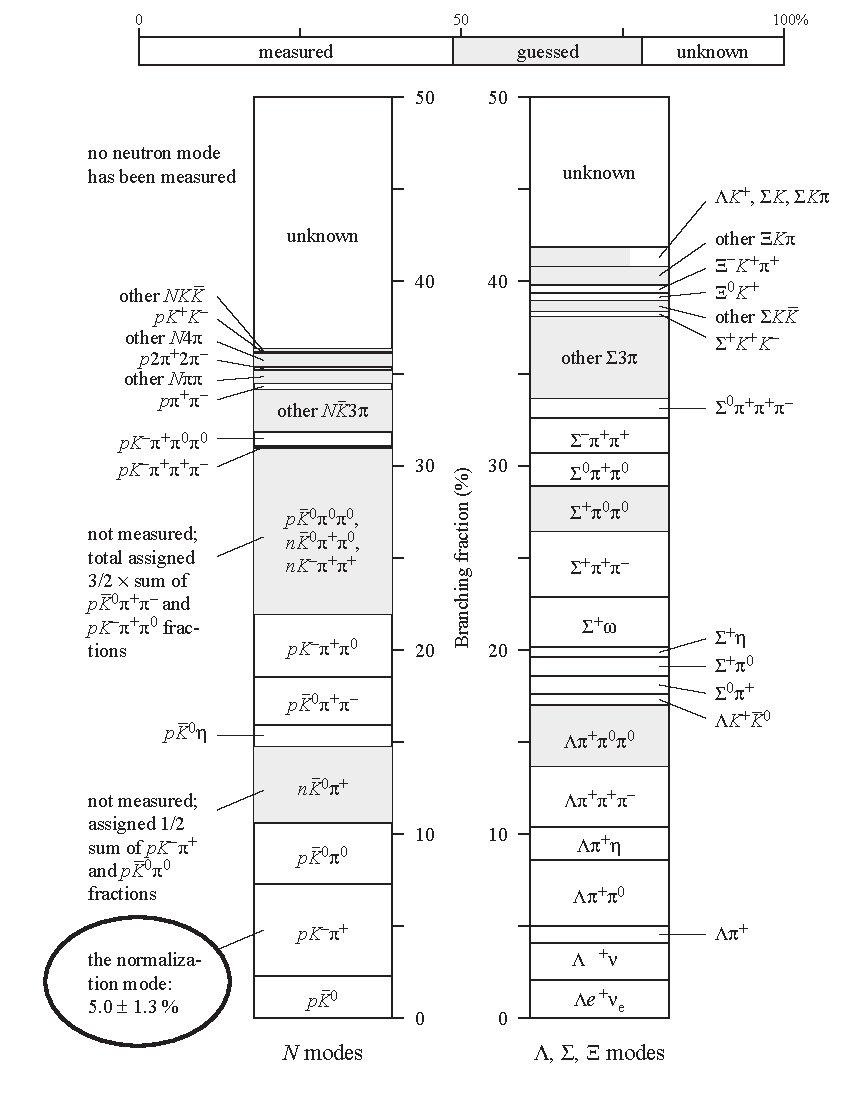
\includegraphics[width=0.45\textwidth]{chap1_br_lambda_c_1.pdf}
 \label{fig:br_lambdac_pdg}
}
\hspace{1pt}
\subfigure[$\mathcal{B}(pK^{-}\pi^{+})$采用Belle测量的结果。]
{
 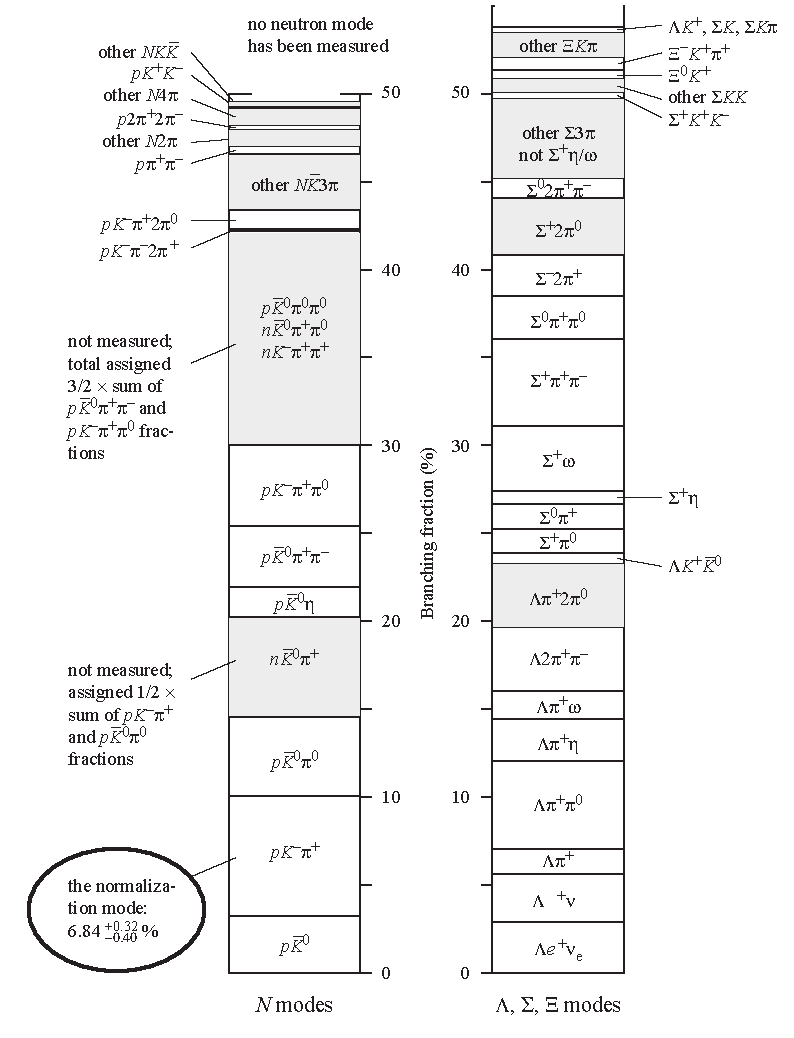
\includegraphics[width=0.45\textwidth]{chap1_br_lambda_c_2.pdf}
 \label{fig:br_lambdac_belle}
}
 \caption{粲重子$\lambdacp$已测量(measured)和未测量(guessed和unknown)衰变分支比大小示意图。}
 \label{fig:br_lambdac}
\end{figure}
从图中我们可以清楚的看到有很多的衰变道没有很好的测量,尤其是末态含有中子的衰变道,基本都是理论预测的结果。
同时我们也注意到这些已知的所有的$\lambdacp$的衰变道的总的分支比远小于1。
这也在一定程度上说明当前的$\mathcal{B}(pK^{-}\pi^{+})$的结果有可能偏低。

Belle实验利用他们在$\Upsilon(nS)$上采取的数据,采用初态辐射的技术在2014年报道了他们测量的$\Lmodeb$的衰变分支比结果$\br{\modeb}=(6.84\pm0.24^{+0.21}_{-0.27})\%$~\cite{Lambdac_belle}。
测量结果的精度达到了$4.7\%$,较PDG2014好了有5倍之多。
这一结果是首次进行的绝对测量, 测量也是模型无关的。
但是我们从图~\ref{fig:bellepaper}~\cite{Lambdac_belle}可以注意到,Belle实验的拟合结果遭受着高本底的污染,这主要是由于其运行在高能量区域所导致的。
\begin{figure}[!tbp]
 \centering
 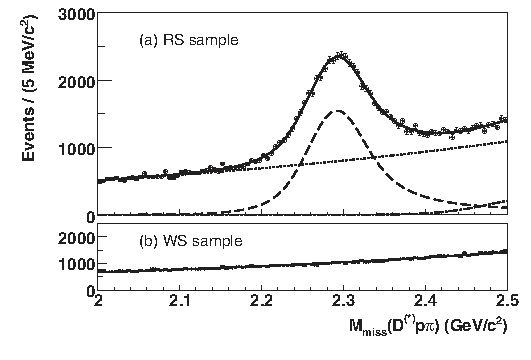
\includegraphics[width=0.8\textwidth]{chap1_belle_paper.pdf}
 \caption[Belle实验的拟合结果图。]{Belle实验的拟合结果图,摘选自文献~\cite{Lambdac_belle}。}
 \label{fig:bellepaper}
\end{figure}
除此之外,高端还遭受着高激发态本底的尾巴的影响,这会大大增加信号数获取的不准确度。
图~\ref{fig:br_lambdac_belle}是采用了Belle的结果$\mathcal{B}(pK^{-}\pi^{+})=(6.84\pm0.24^{+0.21}_{-0.27})\%$来进一步计算之后的$\lambdacp$各个衰变分支比的大小示意图。
我们注意到这些已知的所有的$\lambdacp$的衰变道的总的分支比之和已经超过100\%了。
如果说之前的相对测量是准确的话,那么这在一定程度上暗示Belle的$\mathcal{B}(pK^{-}\pi^{+})$的结果有可能偏高。
BESIII在2016年的时候测量了$\mathcal{B}(pK^{-}\pi^{+})=(5.84\pm0.27\pm0.23)\%$~\cite{Lambdac_bes3},当PDG2016~\cite{PDG2017}合并了BESIII和Belle的结果之后给出$\mathcal{B}(pK^{-}\pi^{+})=(6.35\pm0.33)\%$,从而缓解了Belle测量结果导致分支比超出的问题。


实验上,$\cleo$~\cite{Avery:1993vj}合作组和$\argus$~\cite{Albrecht:1994hr}合作组对于$\Lambda^+_c\to \Xi^{(*)0}K^+$衰变分支比进行过一些测量。
不过这些测量都是20多年前进行的,而且它们都是相对于$\mathcal{B}(\Lmodeb)$的相对测量。它们的测量结果我们同样展示在表~\ref{tab:prediction}中以进行比较。
PDG2016中关于此两个衰变道的结果分别为$\mathcal{B}(\Lambda^+_c\to\Xi^0K^+)=(5.0\pm1.2)\times10^{-3}$~\cite{PDG2017} 和 $\mathcal{B}(\Lambda^+_c\to\Xi^{*0}K^+)=(4.0\pm1.0)\times10^{-3}$~\cite{PDG2017}~\footnote{假定$\Xi(1530)^0\to\Xi^{-}\pi^{+}$的分支比为$\frac{2}{3}$,用它来修正文献~\cite{Albrecht:1994hr}中$\argus$的测量值。}。
BESIII实验利用阈值上的$\ee$湮灭数据去研究$\lambdacp$衰变是更简单更直接的一种方式,这种方式有着其独特的优势所在。
在阈值上$\Lambda_c$是成对产生的,除了$\Lambda_c$对之外不会有额外的任何强子产生。
这就给我们提供了一个非常干净的$\Lambda_c$的产生环境。
此外,由于是成对产生,我们可以双标记的技术来进行测量。
这样一来,双标记侧几乎是没有本底的,结果更加可靠。
另外一个就是双标记方法可以做到绝对测量,单标记的系统误差基本可以认为消除掉了。这也是阈值上数据的优势。
基于BESIII在 $\sqrt{s}=4.6\gev$ 处采集的567\,pb$^{-1}$的$\ee$对撞数据,运用成熟的双$\Lambda_{c}$标记技术我们可以对$\mathcal{B}(\Lambda^+_c\to \Xi^{(*)0}K^+)$进行首次的绝对测量。

\section{重夸克偶素产生的研究现状}
\subsection{重夸克偶素简介}

重夸克是指粲夸克($c$)、底夸克($b$)和顶夸克($t$),他们都比较重,尤其是顶夸克$t$特别的重,寿命在$10^{-13}$量级上,几乎来不及形成强子。
重夸克偶素~\cite{Lansberg:2008gk}是指带有各种$J^{PC}$ 量子数的$c\bar{c}$和$b\bar{b}$ 束缚态,其中$J^{PC}$由两个组合重夸克的总自旋S和总角动量L决定。
重夸克偶素的物理过程涉及了QCD的所有能区。
在高能区偶合常数是可适用的,QCD 微扰展开易于收敛;而到了低能区域,非微扰是主导的,QCD失效了,只能通过其他非微扰方法来处理~\cite{Kramer:2001hh}。
重夸克偶素物理过程的研究对考察微扰与非微扰QCD交叠区域的动力学,检验和发展QCD 模型起着重要意义。
在过去的三十多年里,许多理论工作也验证了QCD在重夸克偶素上的应用。
历史上比较流行的理论基本上有三种:色单态机制(CSM)、 色蒸发模型 (CEM)、 色八重态机制(COM)。
伴随着实验的进程,人类已经提前对QCD有了一个很好的理解。
理论计算和实验都在夸克偶素的产生上做出了很大的贡献,然而还存在着很多问题~\cite{Brambilla:2010cs}。
例如,色单态模型在解释Tevatron上正反质子对撞实验中高横动量$\pt$下$\jpsi$ 粒子的产生截面时遇到了很大的困难,产生了数量级上的差异。
COM应用了1986 年被Caswell 和Lapage 发展起来的有效场论发展出了非相对论量子色动力学(Non-Relativistic QCD,NRQCD),
目前成为主流的描述强产生的里面模型,在高$\pt$区域描述的比较好。
虽然NRQCD能够很好地解释实验上测得的重味夸克偶素的产生截面,但极化预测值与CDF 实验所测结果相矛盾~\cite{Lansberg:2008gk}。
COM 和领头阶(LO) CSM理论,预言了高横动量下重夸克偶素的极化,但是不能解释强子对撞中$\psi(nS)$ 和$\Upsilon(nS)$ 的极化。
基于非微扰QCD框架开发的Fixed-Order-with-Next-to-Leading-Logarithm (FONLL)~\cite{Cacciari:1998it}成功的用于描述多个非直接产生的重夸克偶素态的产生截面。

\subsection{$\lhcb$上重夸克偶素的研究}

大型强子对撞机$\lhc$上,在质子质子对撞为2.76$\tev$,7$\tev$,8$\tev$和13$\tev$的质心系能量下,$\atlas$、$\cms$、$\alice$ 和$\lhcb$四个实验都对夸克偶素进行过研究。
我们接下来以$\lhcb$实验上$\jpsi$和$\psitwos$在7$\tev$质心系能量下为例介绍目前对重夸克偶素的产生截面测量以及极化测量情况。

在高能对撞实验上,以粲夸克偶素为例(图\ref{fig:charmonium} 给出了按照$J^{PC}$和质量总结的各个粲偶素和类粲偶素粒子),其产生主要有三种来源:部分子碰撞直接产生,高激发态退激发产生以及$b$强子衰变产生。
\begin{figure}[!tbp]
\begin{center}
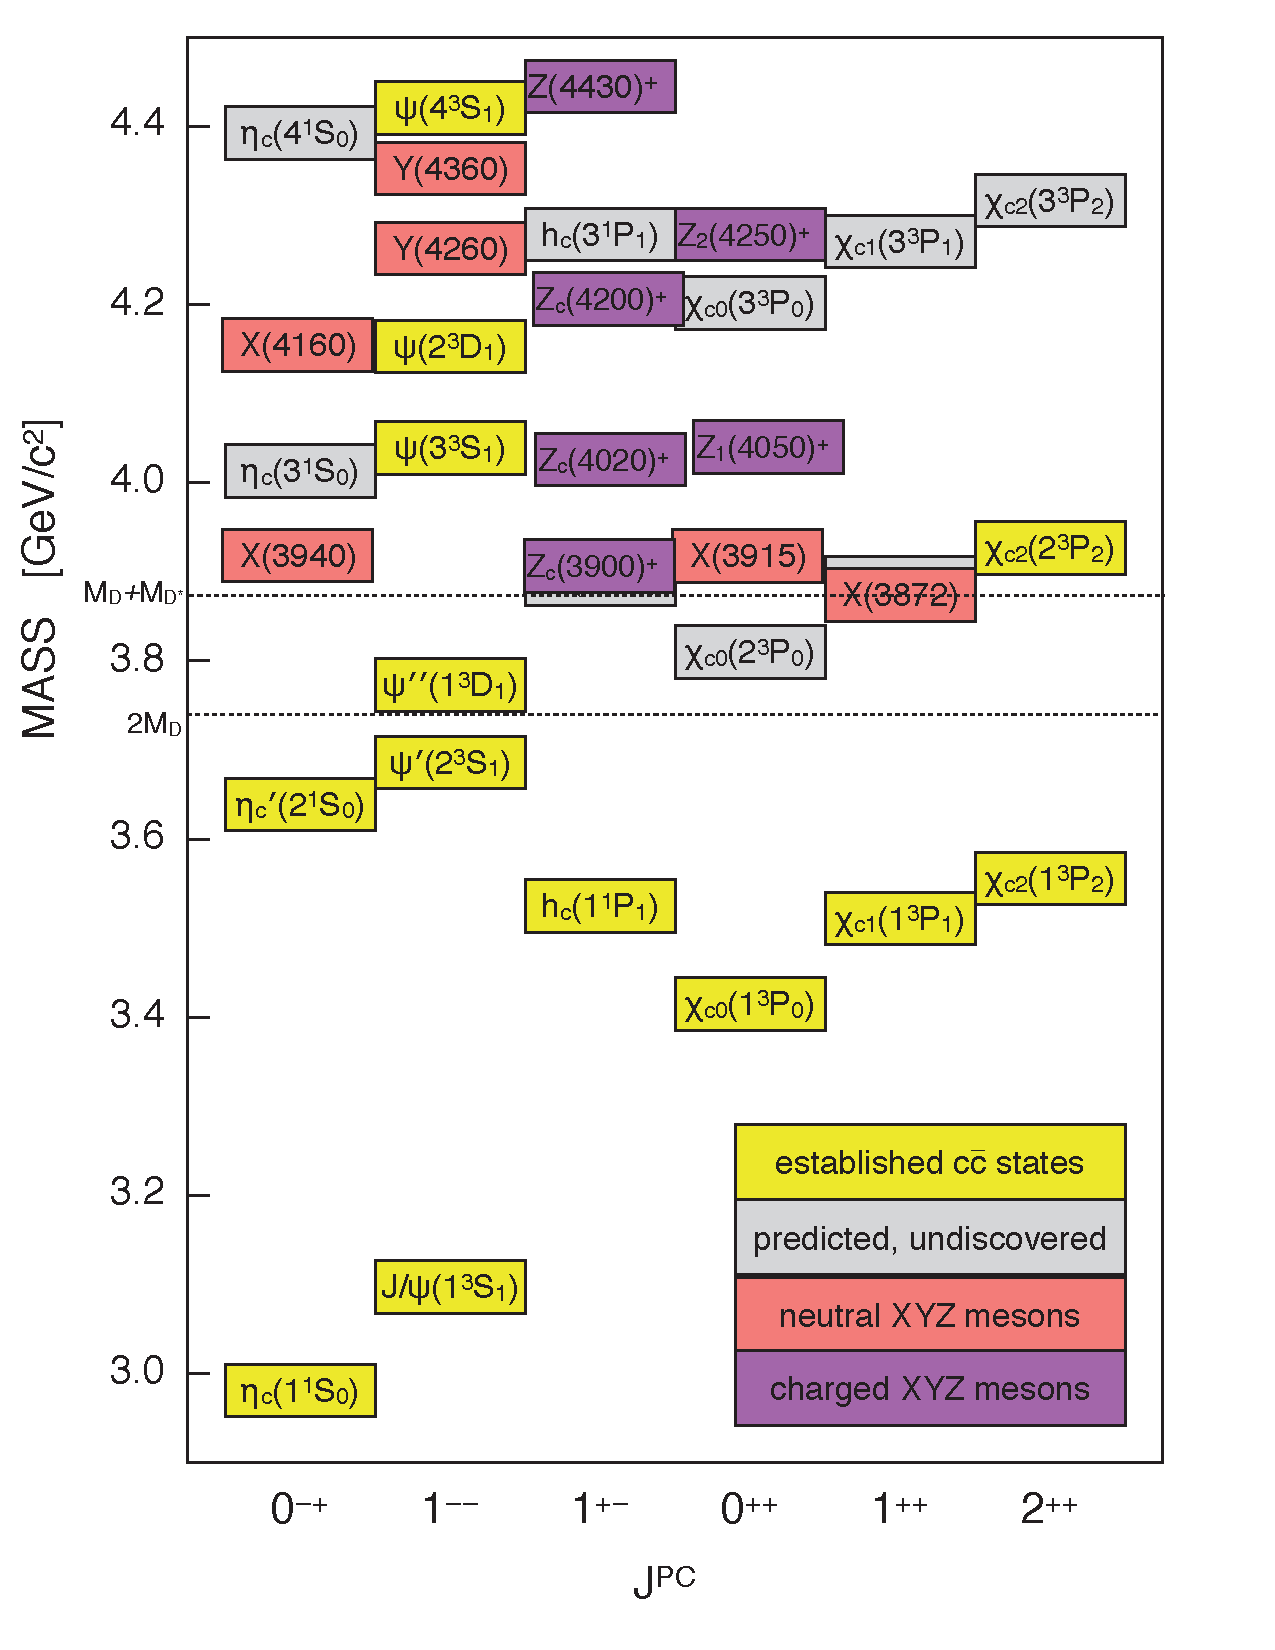
\includegraphics[width=0.85\textwidth]{chap1_charmonium.pdf}
\end{center}
\caption{粲偶素和类粲偶素粒子分布示意图。}
\label{fig:charmonium}
\end{figure}
$\lhcb$实验在运动学区间$y\in$[2.0,4.5]和$\pt\in$[0,14]$\gev$内,对单举$\jpsi$微分产生截面,包括直接产生的和来自$b$强子衰变来的都进行了测量~\cite{Aaij:2011jh}。
对$\psitwos$的测量由于采用了多个重建衰变道,其研究的运动学区间为$y\in$[2.0,4.5]和$\pt\in$[0,14]$\gev$~\cite{Aaij:2012ag}。
同样,对于直接产生的$\psitwos$和来自$b$强子衰变来的$\psitwos$都进行了测量。
如图~\ref{fig:jpsi7TeV}和图~\ref{fig:psitwos7TeV}所示,
在高动量区范围内,NLO NRQCD理论计算与$\lhcb$的测量吻合的很好。
来自$b$强子衰变的$\jpsi$/$\psitwos$的微分截面测量结果与FONLL的预言符合的很好。

\begin{figure}[!tbp]
\centering
\begin{minipage}[t]{0.49\textwidth}
\centering
\includegraphics[width=1.0\textwidth]{chap1_jpsi7TeV_prompt}
\end{minipage}
\begin{minipage}[t]{0.49\textwidth}
\centering
\includegraphics[width=1.0\textwidth]{chap1_jpsi7TeV_bdecay}
\end{minipage}
\caption{质子质子对撞直接产生的$\jpsi$和$b$强子衰变而来的$\jpsi$在7$\tev$下产生截面随着$\pt$的变化。左图为直接产生的$\jpsi$和NRQCD模型计算的对比。右图为$b$强子衰变而来的$\jpsi$与FONLL模型的结果比较。}
\label{fig:jpsi7TeV}
\end{figure}


\begin{figure}[!tbp]
\centering
\begin{minipage}[t]{0.49\textwidth}
\centering
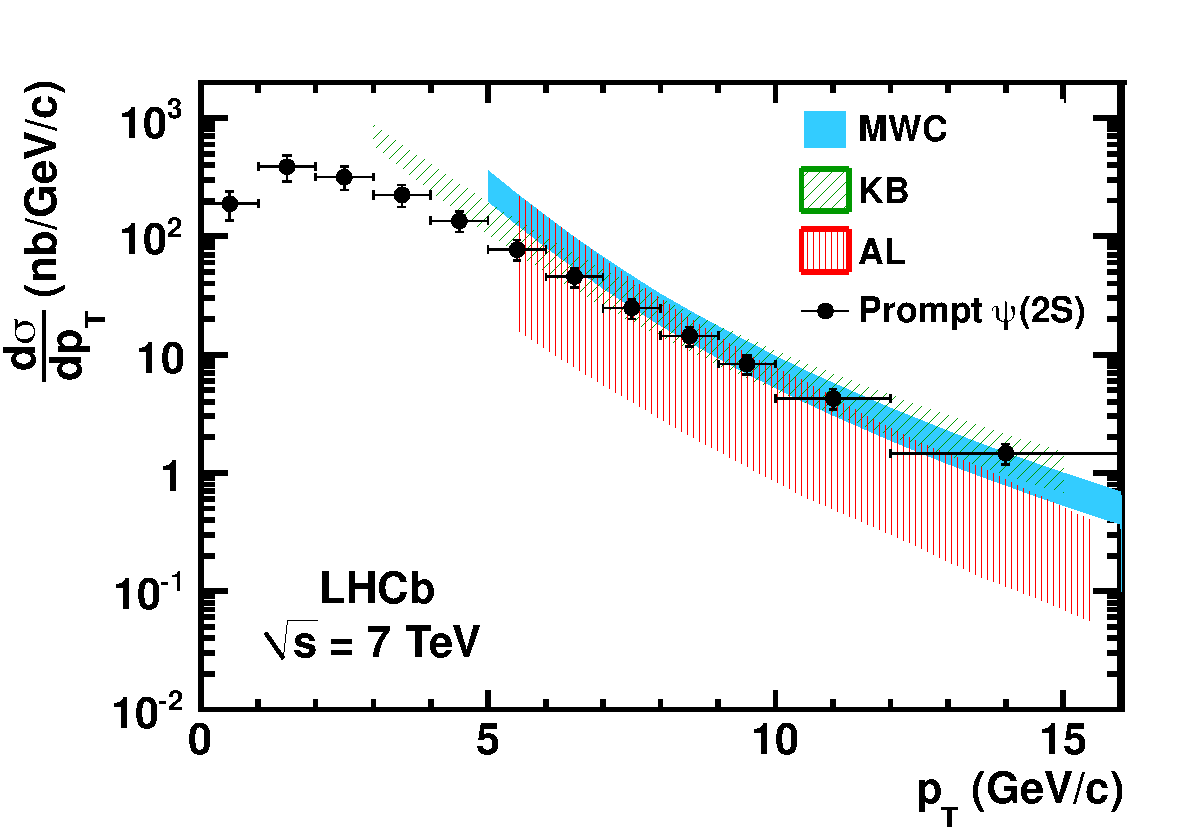
\includegraphics[width=1.0\textwidth]{chap1_psitwos7TeV_prompt}
\end{minipage}
\begin{minipage}[t]{0.49\textwidth}
\centering
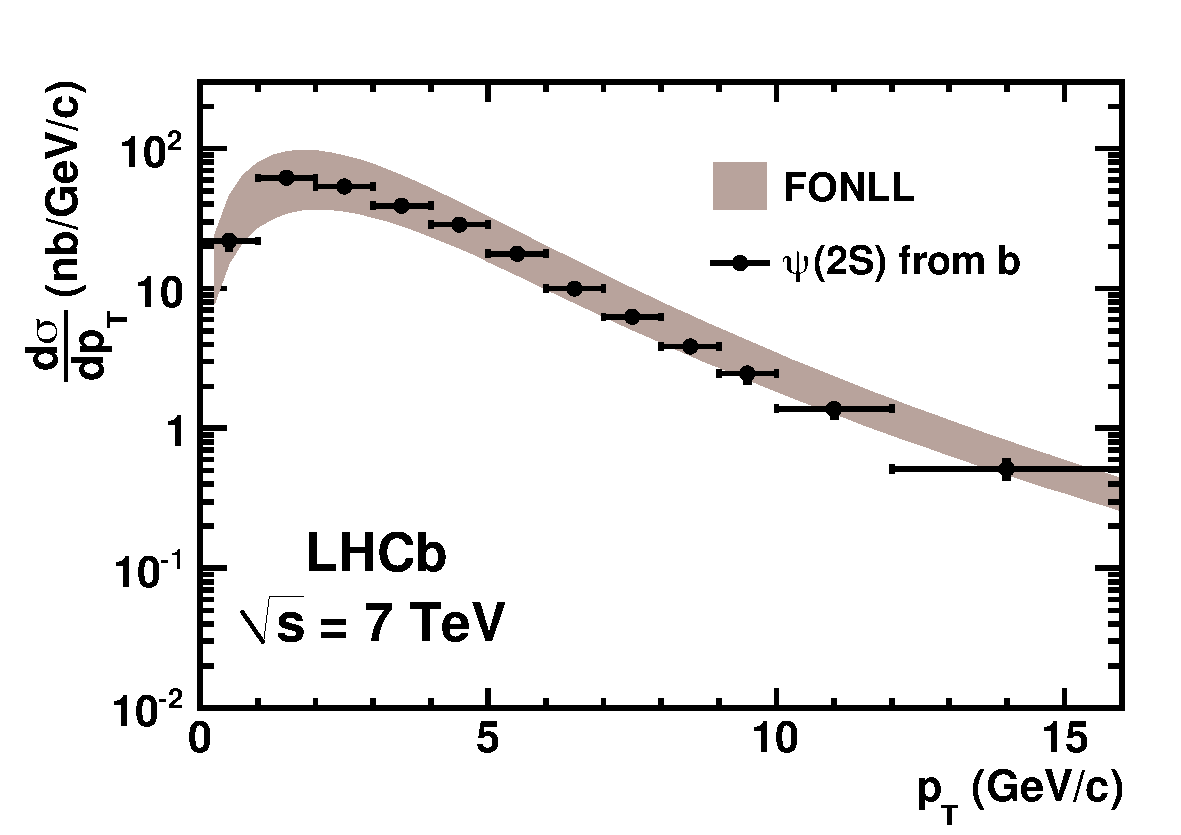
\includegraphics[width=1.0\textwidth]{chap1_psitwos7TeV_bdecay}
\end{minipage}
\caption{质子质子对撞直接产生的$\psitwos$和$b$强子衰变而来的$\psitwos$在7$\tev$下产生截面随着$\pt$的变化。左图为直接产生的$\psitwos$和三种NRQCD模型计算的对比。右图为$b$强子衰变而来的$\psitwos$与FONLL模型的结果比较。}
\label{fig:psitwos7TeV}
\end{figure}

%$\cms$测量了$\Upsilon(nS)$~\cite{Chatrchyan:2012woa}的极化,在误差范围内重夸克偶素没有大的纵向和横向极化。
%$\alice$对$\jpsi$ ~\cite{Abelev:2011md}的极化测量同样表明,在误差范围内夸克偶素没有大的纵向和横向极化。
%
2011年,$\lhcb$ 探测器采集了大约1.0 fb$^{-1}$的质心能量为7 $\tev$ 质子质子对撞的数据。
利用其中约370 pb$^{-1}$的数据,分别在螺旋度参考系和Collins——Soper 参考系,在不同的横动量和快度区间,测量了直接产生的$\jpsi$ 粒子的三个极化参数$\lambda_{\theta}$、$\lambda_{\theta\phi}$ 以及$\lambda_{\phi}$。
在运动学区间2$<\pt<15\gev$,2.0$<y<$4.5,在螺旋度参考系中$\lambda_{\theta}$最小边界$\simeq$ $-$0.2,具有轻微的纵向极化并且随着$\jpsi$ 横动量和快度的增加稍微减少,而$\lambda_{\theta\phi}$和$\lambda_{\phi}$ 在误差范围内近似为0。
利用全部1.0 fb$^{-1}$的数据,$\lhcb$还在螺旋度参考系和Collins——Soper 参考系中测量了直接产生的$\psitwos$的极化参数。
测量结果表明,在误差范围内,在大部分运动学区间$\psitwos$的三个极化参数都近似0,而在某些区域$\psitwos$有轻微的纵向极化,$\lambda_{\theta}$处于$-$0.2到0之间。
如图~\ref{fig:polarization}所示,直接产生的$\jpsi$和$\psitwos$在7$\tev$下极化参数$\lambda_{\theta}$随着$\pt$的变化,并和CSM模型以及三种NRQCD模型计算进行了对比。
结果表明,在$\lhcb$上$\jpsi$和$\psitwos$并不具有很大的横向极化或者纵向极化。
在$\lhcb$和$\alice$探测器共同覆盖的运动学区间内,$\jpsi$的测量结果和$\alice$结果在误差范围内是一致的。
$\lhcb$关于$\jpsi$和$\psitwos$的极化测量不支持领头阶CSM或者NRQCD的理论预言。
目前为止,无论哪种模型都不能同时很好的描述重夸克偶素的微分产生截面和极化~\cite{Knuenz:2015hga},重夸克偶素至今仍然是研究的热点和难点。


基于$\lhcb$在$\sqrt{s}=13\tev$ 处采集的275\,pb$^{-1}$~的$\pp$对撞数据,我们可以在高能量下测量$\psitwos$介子的微分产生截面。
这是在$\lhcb$上7$\tev$质心能量下测量后进行的又一次$\psitwos$微分产生截面的测量。测量采用的大统计量的真实数据保证了测量的更高精度,
测量结果可以很好的检验现有理论模型计算的可靠程度。
结果中对微分产生截面与7$\tev$下$\psitwos$发表结果的比值进行了研究,由于7 $\tev$下$\psitwos$只是发表了随$\pt$ 的变化,所以比值结果只是给出了随$\pt$的变化。
与13$\tev$ 下$\jpsi$结果的比较,可以研究比值随横动量$\pt$、和快度$y$的变化情况。

\begin{figure}[!tbp]
\centering
\begin{minipage}[t]{0.49\textwidth}
\centering
\includegraphics[width=1.0\textwidth]{chap1_polarization_jpsi}
\end{minipage}
\begin{minipage}[t]{0.49\textwidth}
\centering
\includegraphics[width=1.0\textwidth]{chap1_polarization_psitwos}
\end{minipage}
\caption{7$\tev$下极化参数$\lambda_{\theta}$随着$\pt$的变化。左图为直接产生的$\jpsi$和CSM模型以及三种NRQCD模型计算的对比。右图为直接产生的$\psitwos$和CSM模型以及三种NRQCD模型计算的对比。}
\label{fig:polarization}
\end{figure}


\section{论文结构}
	本论文结构如下:第一章介绍本论文相关的理论和实验现状,交待选题背景。
	第二章介绍北京正负电子对撞机~BEPCII 和北京谱仪~BESIII。
	第三章介绍BESIII上粲重子$\Lambda^+_c\to \Xi^{(*)0}K^+$的绝对衰变分支比测量。
	第四章详细介绍$\lhcb$上13$\tev$下$\psitwos$介子微分产生截面的测量。
	第五章为总结和展望。
